\documentclass[a4paper,12pt]{article}
\usepackage[hmargin=2.5cm,vmargin=2.5cm]{geometry}

\usepackage[utf8]{inputenc}   % le fichier .tex est en UTF-8     
\usepackage[francais]{babel}  %typo française                    
\usepackage[T1]{fontenc}      % encodage des fonts latex         
\usepackage{lmodern}                                             
\usepackage{microtype}        % typo supplémentaires             



\usepackage{graphicx} %inclusion de graphiques


\usepackage{hyperref} % liens dans le pdf
\hypersetup{%
  pdftitle={Title},
  pdfauthor={Author1, Author2},
  pdfkeywords={keywords}
  pdfsubject={article},
  colorlinks=true,
  linkcolor=black,
  urlcolor=black,
  citecolor=black
}


\title{1CKA dépliée,epsilon=16} % c'est la déclaration



\begin{document}

\maketitle % c’est ici que le titre est inséré


    Les 10000 séquences uniques de meilleurs énergies Monte-Carlo.
    Les énergies de références: GBE4SA.

  
  \begin{sffamily}
    
   \begin{figure}[!htbp]
     \centering
     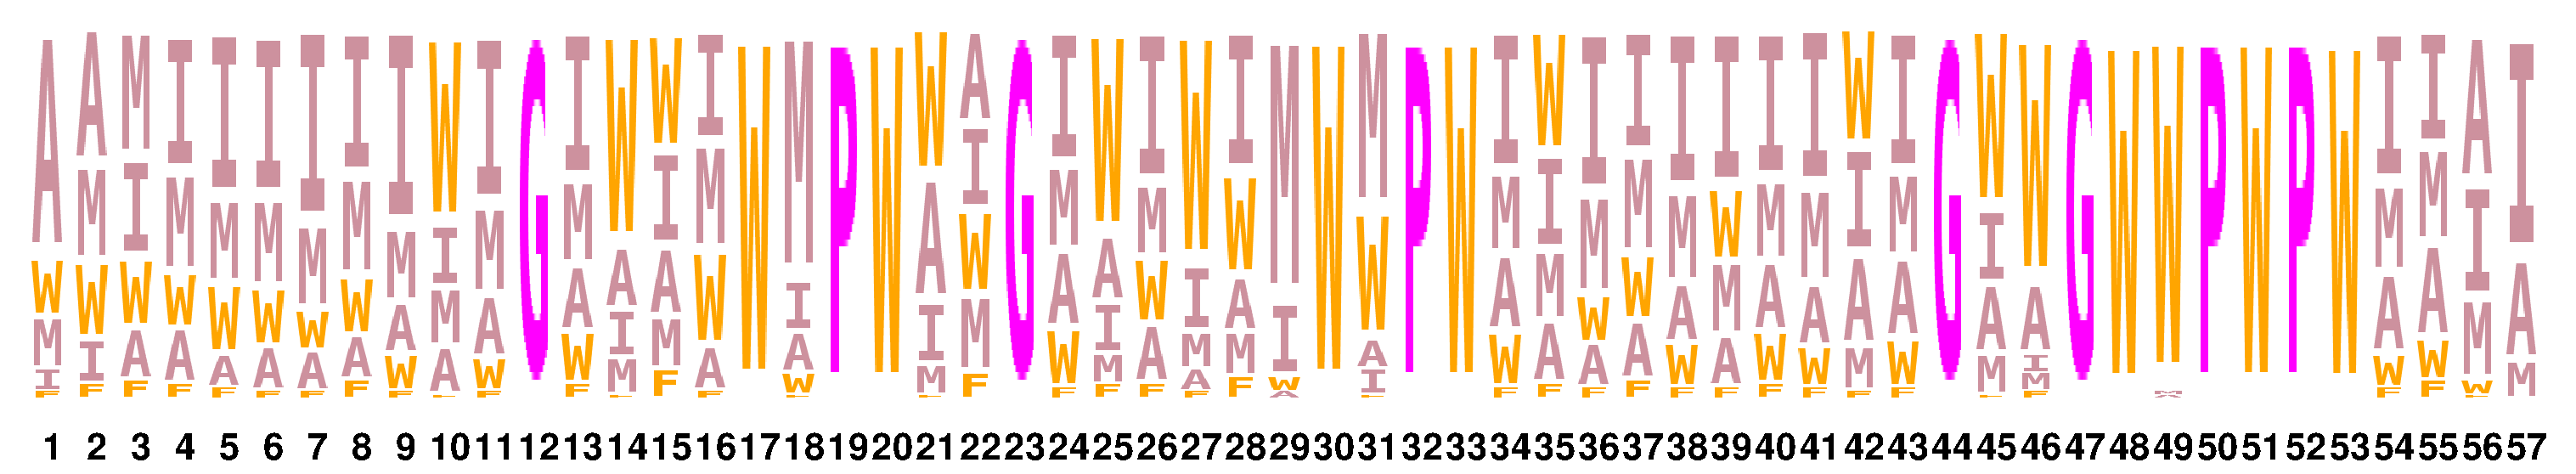
\includegraphics[width=18cm]{1CKAe16.eps}
     \begin{bfseries}
      \resizebox{18cm}{3mm} {
        \begin{tabular}{*{57}{c}}
          2.5 & 2.9 & 2.5 & 2.4 & 2.3 & 2.3 & 2.0 & 2.4 & 2.1 & 2.6 & 2.2 & 1.0 & 2.5 & 2.6 & 2.9 & 2.5 & 1.1 & 1.8 & 1.0 & 1.0 & 2.9 & 2.9 & 1.0 & 2.6 & 2.6 & 2.5 & 2.2 & 2.7 & 1.3 & 1.1 & 2.4 & 1.0 & 1.0 & 2.5 & 2.8 & 2.2 & 2.5 & 2.3 & 2.5 & 2.5 & 2.3 & 2.9 & 2.5 & 1.0 & 2.8 & 2.2 & 1.0 & 1.0 & 1.2 & 1.0 & 1.0 & 1.0 & 1.0 & 2.4 & 2.6 & 2.4 & 1.9 \\
      \end{tabular}
      }
     \end{bfseries}
     \caption{Séquence logo et exponentiel de l'entropie pour une température de 0,3}
     \label{fig-seqlogo-T=03}
   \end{figure}

  \end{sffamily}
\end{document}
